% Created 2014-05-08 四 21:40
\documentclass[10pt,b5paper]{article}
\usepackage{graphicx}
\usepackage{xcolor}
\usepackage{xeCJK}
\usepackage{longtable}
\usepackage{float}
\usepackage{textcomp}
\usepackage{geometry}
\geometry{left=0cm,right=0cm,top=0cm,bottom=0cm}
\usepackage{multirow}
\usepackage{multicol}
\usepackage{listings}
\usepackage{algorithm}
\usepackage{algorithmic}
\usepackage{latexsym}
\usepackage{natbib}
\usepackage{fancyhdr}
\usepackage[xetex,colorlinks=true,CJKbookmarks=true,linkcolor=blue,urlcolor=blue,menucolor=blue]{hyperref}


\usepackage{CJKutf8}
\begin{CJK}{UTF8}{gbsn}
\lstset{language=c++,numbers=left,numberstyle=\tiny,basicstyle=\ttfamily\small,tabsize=4,frame=none,escapeinside=``,extendedchars=false,keywordstyle=\color{blue!70},commentstyle=\color{red!55!green!55!blue!55!},rulesepcolor=\color{red!20!green!20!blue!20!}}
\author{Heyan Huang}
\date{\today}
\title{CS572 Project 4 Report}
\hypersetup{
  pdfkeywords={},
  pdfsubject={},
  pdfcreator={Emacs 24.3.50.1 (Org mode 8.2.5h)}}
\begin{document}

\maketitle
\tableofcontents

\begin{abstract}
Steady-state genetic algorithm is applied to the Schwefel function. For this project, I chose the population size of 100, sample size of 10, applied Tournament selection method to select 2 elite parent as the regularly-based method, and using the Roulette wheel selection method with fitness sharing as the opposite choice. In each of my new generation, I kept a version of my elite parent, then 2-point crossover with crossover rate of 0.9, mutated the 2 individuals in each representation dimension with mutation rate of 0.5. And I replaced the worst 2 individuals in previous generation with the mutated 2 individuals. I repeated the process until find good solution. To compare the two methods for the Schwefel function scientifically, because of the randomness of population generation, I have used single individuals comparison, 100 repeats comparison and 300 repeats comparison in order to get reasonable results. And the results shows that when there are sufficient generation runs, the fitness sharing method in general performs better than the regularly-based Tournament selection method. But if the generation count is not enough, the Tournament selection method performs better. 
\end{abstract}

\begin{center}
\begin{tabular}{ll}
\hline
algorithms & Steady-state\\
\hline
Population Size & 100\\
Selection Method & Tournament rank-based Selection sample size of 10 vs\\
Selection Method & Roulette Wheel fitness-based selection with fitness sharing, $\delta$$_{\text{share}}$=10.24, $\alpha$=0.5\\
Elitism(if used) & Yes, one copy of parent though not necessary just to speed up the processes\\
Crossover Method & two-point crossover\\
Crossover rate & 0.9\\
Mutation Method & mutate each representation dimension with mutation rate of 0.5\\
Fitness function & the Schwefel function to evalate the points\\
\hline
 & By using 100 \& 300 repeats with different population size and generation count\\
Results & combinations, fitness sharing does help in Schwefel function for finding the\\
 & global optima by getting smaller fitness faster.\\
\hline
\end{tabular}
\end{center}

\section{Program Design \& Data Structures}
\label{sec-1}
\begin{itemize}
\item In this project, I have implemented Object-Oriented (OO) design as suggested by Dr. Soule.
\item There are three classes, Function, Individual and Population.
\item Function object packs the threshold values and fitness functions all together for any of the six functions which has been used in project 1; Functions are classified into two categories, Separable and inseparable. The essential things be able to packs functions are the two different categories of function pointers which will later be used for calculating the fitness for each individual.
\item Individual object sets pointer to Function instance, and also generate initial values, builds solution representation;
\item Population object sets pointer to an array of individuals and define the necessary genetic algorithm functions like 2-point crossover, builds new generation.
\item The main.cpp program linked all these objects together and solves the problems.
\end{itemize}
\section{Algorithm Descriptions}
\label{sec-2}
\subsection{Genetic Algorithm}
\label{sec-2-1}
In this Project, since I am trying to implement an OO design together with handling pointer, to try to avoid complexity and also considering my laptop CPU limitations, I chose to use the easier to implement Steady-state Algorithm at the cost and risk of slowing down and may not get the expected Results within limited time frame.

My genetic algorithm essential steps are listed as followed:
\begin{itemize}
\item Instance a Population object of Population size 100;
\item Using Tournament rank-based selection method selected sample size of 10 individuals during each generation; Compare sample fitnesses and keep the best two elite individuals untouched into the new generation.
\item As comparison, for Roulette Wheel Selection method with fitness sharing, I calculated the individuals' fitness and shared fitness, and select the two parent by randomly generated probabilities, which would result in high shared fitness individuals will be more likely to be selected as parent compared with low shared fitness individuals. Keep two selected one as the parent for the new generation.
\item Trying to speed up the evolution, I replaced the worst two individuals in each parent generation with the 2-point crossover and mutated version of previously found sample elite individuals. Crossover and mutations are done with specific crossover rate (in this project 0.9) and mutation rate (in this project 0.5 for each dimension representation).
\item I loop through these steps trying to approach the final steady state. Loop will eventually end when best individual gets the fitness less than 0.0001.
\end{itemize}

The pseudo-algorithm is listed followed:  
\begin{lstlisting}[language=c++]
Generate a population of size 100

Loop until best individual reaches threshold fitness value
    record the best individual index, representation \& fitness

    set sample size = 10
    set crossover rate = 0.8
    set mutation rate = 0.5

    loop do

        // pick elite 2 individuals from random sample, Tournament method
        randomly select a sample of 10, save Population indexes as value
        winner Fitness = Sample[0].fitness
        winner index = sample[0]
        second Fitness = winner Fitness
        second index = winner index
        Loop ( sample size - 1 ) times
            temp Fitness =  Sample[i].fitness;
            if temp Fitness better than winner Fitness
                second Fitness = winner Fitness
                second index = winner index
                winner Fitness = temp Fitness
                winner index = temp index
            if temp fitness worst than winner Fitness and
               temp fitness better than second Fitness
                second Fitness = temp Fitness
                second index = temp index
        return struct {winner index, second index} as twoIdx

        // Get worst 2 individual indexes from Population:  
        worst Fitness = Population[0].fitness
        worst index = 0
        second Fitness = worst Fitness
        second index = worst index
        Loop population size -1 times
            temp Fitness = Population[i].fitness;
            if temp Fitness worst than worst Fitness
                second Fitness = worst Fitness
                second index = worst index
                worst fitness = temp Fitness
                worst index = temp index
            if temp fitness better than winner Fitness and
               temp fitness worse than second Fitness
                second Fitness = temp Fitness
                second index = temp index
        return struct {worst index, second index} as twoIdx

        // keep elite parent into new generation untouched
        copy parent representations into worst individuals positions
        winfst = sample winner first
        winsnd = sample winner second
        fst = population worst first
        snd = population worst second
        Loop number of dimension p times
            popu[fst].point[i] = popu[winfst].point[i]
            popu[snd].point[i] = popu[winsnd].point[i]
            popu[fst].fitness = popu[winfst].fitness
            popu[snd].fitness = popu[winsnd].fitness

        // 2-point crossover parent with crossover rate
        generate random float number
        if random value greater then crossover rate
            do nothing and end of this step
        else
            generate two indexes within range [1, p-2] and not equal, lowIdx, highIdx
            allocate temporary float memory space of size (highIdx-lowIdx)
            copy second parent middle fragment to temporary space
            copy first parent middle fragment into second parent middle positions
            copy temporary fragment into first parent middle positions

        // mutate the crossover parent with mutation rate
        calculate divider corresponding to generation counter
        extract Function specific low threshold value low
        extract Function specific high threshold value high
        allocate temporary float space for store mutated value
        Loop number of dimension p times
            generate random float number
            if random value less then mutation rate
                generate random value delta corresponding to Function range and divider    
                apply increase or decrease to current dimension \&
                store the result in temporary float space
                check, repeat \& make sure mutated value is valid
            copy from temporary space to original dimension value position
        calculate new fitness value for mutated Individual    
        repeat above loop one more time for the other crossover individual

        // generate new child Population
        by conduct above three main modules, it is currently new generation already

    End loop
\end{lstlisting}
\subsection{Initial Random Solution Generation}
\label{sec-2-2}
Initial random solutions are the solutions we randomly generated to start and begin our evolutionary process. According to different function problem requirements, any random start point must have all the valid values for 30-dimension. So as far as the randomly generated points are within the valid value range, and as far as any value in the valid range has equal probability to get generated, which means our random generator can produce any valid value within range with equal probability and has no bias to weaken our tests, we are good to go.

The initial random solutions are coded in the "individual.h" interface, necessary codes are listed below:
\begin{lstlisting}[language=c++]
typedef float (*funPtrSep)(float);       // separable
typedef float (*funPtrNSe)(float*, int); // inseparable

class Function {
 public:
    Function(float l, float h, funPtrSep ptr, bool flag);
    Function(float l, float h, funPtrNSe ptr, bool flag);
    float low;
    float high;
    float fitness;
    bool sepaFlag;
    funPtrSep sepPtr;
    funPtrNSe nsePtr;
};

class Individual {
 public:
    Individual(Function* funptr);                    
    // functions
    void generate();   // generate an individual
    float getFitness();// calculate the fitness when initialization
    float* point;      // pointer to dynamic array of dimension size p (constant)
    float fitness;     // store fitness value for the point
    float mutRate;
    Function* funPtr;
};

void Individual::generate() {           
    int high = (int)((*funPtr).high);
    if (high < (*funPtr).high)
        high = high + 2;
    for (int i = 0; i < p; ++i) {
        if ( (rand()%100/100.0) >= 0.50 )
            point[i] = rand() % high - (rand() % 100000)/100000.0;  // pos
        else
            point[i] = -rand() % high + (rand() % 100000)/100000.0; // neg
        // check if value is within valid range for specific function
        while (point[i] < (*funPtr).low || point[i] > (*funPtr).high) {
            if ( (rand()%100/100.0) >= 0.50 )
                point[i] = rand() % high - (rand() % 100000)/100000.0;
            else
                point[i] = -rand() % high + (rand() % 100000)/100000.0;
        } // while
    }     // for
    fitness = getFitness(); // caculate the fitness for the point
}
\end{lstlisting}
\subsection{Representation}
\label{sec-2-3}
Each solution is represented by a 30-dimension dynamically allocated float array storing the float values for the corresponding dimensions, together with a float value storing the fitness float results for that solution.

Solution representation is defined in "individual.h" interface. Corresponding codes are included as followed:
\begin{lstlisting}[language=c++]
class Individual {
 public:
    Individual(Function* funptr);                        
    float* point;  // pointer to dynamic array of dimension size p (constant)
    float fitness; // store fitness value for the point
};
\end{lstlisting}
\subsection{Fitness function}
\label{sec-2-4}
Fitness function is the particular objective function that is used to measure and summarise how good the current solution is to achieve the global optimum. For this project, we have six different fitness functions. Each of them is independent of any of the other.

The Schwefel Function's fitness function is represented below:
\begin{math}
\noindent
\\ f_{Sch}(x) = 418.9829*p + \sum\nolimits_{i=1}^{p} x_i*sin(\sqrt{|x_i|})
\end{math}

Since each of our point/solution has 30-dimension, we plug the point array values into these fitness functions specifically, that way we would be able to get the fitness for the solution.
\begin{itemize}
\item For separable Schwefel function, the fitness function is originally defined at dimension layer, and then at the point layer, I simply sum the fitness of 30-dimension all together to get the point fitness because the function is separable.
\item Dimension layer functions are defined in the "fitness.h" interface, and point layer functions are defined in the "individual.h" interface. Mythologically speaking, the point layer definition is simply loop and call the dimension layer functions through all the 30-dimension.
\end{itemize}

Take Schwefel function as the example, necessary codes are listed as followed: 
\begin{lstlisting}[language=c++]
const float schl = -512.0300; 
const float schh = 511.9700; 
float getSchFitness(float x);

float getSchFitness(float x) {   // dimension-layer fitness
    float y = 418.9829;
    if (x - 0.0 < 0.000000001) 
            y = y + x*sin(sqrt(-x));
    else
            y += x*sin(sqrt(x));
    return y;
}

float Individual::getFitness() { // point-layer fitness
    float y = 0;
    if ((*funPtr).sepaFlag)      // if separatable functions
        for (int i = 0; i < p; ++i) 
            y += funPtr->getFitness(point[i]);          
    else                         // non separatable functions   
        y = funPtr->getFitness(point, p);
    fitness = y;
    return y;
}
\end{lstlisting}
\subsection{Fitness Sharing Function}
\label{sec-2-5}
The fitness sharing function requires to calculate each individual's fitness in the population first, and then calculate the distance among individuals. And based on the distance and shared fitness we use Roulette wheel selection method to select two parent for the new generation. 

The fitness sharing function is expressed as below: 
\begin{math}
\\  f_{sharing}(i) = \frac{population[i].fitness}{\sum\nolimits_{j=0}^{popSize-1} Sh(distance(i, j))}
\\ and 
\\ Sh(d) = \left\{
\begin{array}{l l}
0 & \quad \text{if\ (d > \delta_{share})}\\
1 - (\frac{d}{\delta_{share}})^{\alpha} & \quad \text{if\ (d <= \delta_{share})}
  \end{array} \right.\]
\\ and 
\\ d(i, j) = \sqrt[2]{\sum\nonlimits_{p=0}^{29} (population[i].point[p] - population[j].point[p])^2}
\end{math}

So to calculate the shared fitness, upon the individual's fitness we have got already, we need go one more step to calculate the relative distance of each individual to other population members. If two individuals' distance is larger than the limits ($\delta$$_{\text{share}}$), we set the shared distance among the two to be 1, otherwise calculate it differently as listed above. 

In this project, the parameters I have used for this project are suggested by Dr. Soule, and the $\delta$$_{\text{share}}$ = 10.24, which is about 1\% of the valid function value range, and $\alpha$ = 0.5.

The function code to calculate the shared fitness for each individual is listed below as reference:
\begin{lstlisting}[language=c++]
void Population::distance(int x) {
    dist[x] = 0.0;
    float tmp = 0.0;
    for (int i = 0; i < size; ++i) {
        for(int j = 0; j < p; ++j) 
            tmp += pow((popu[i].point[j]-popu[x].point[j]), 2);
        tmp = sqrt(tmp);
        if (tmp - 10.24 >= 0.000001)
            tmp = 0.0;
        else
            tmp = 1 - pow(tmp/10.24, 1);
        dist[x] += tmp;
    }
    fitshare[x] = (float)(popu[x].fitness/dist[x]);
}
\end{lstlisting}
\subsection{Selection}
\label{sec-2-6}
Since two of the most widely used selection methods are covered during class, Tournament selection method and the Roulette wheel selection method. Generally speaking, the Roulette wheel selection method is a weight or rank based selection, so applying this method could potentially easily result in over-selection or under-selection. In over-selection, the best individuals would be able to dominant the offspring quite often. While in situations when all the individuals are equally likely to be selected, it could easily ended up with under-selection.

On the other side, the Tournament selection is completely random. By selecting a certain size of sample from the population, we would be able to compare the fitness among the sample. And we select the best two as the parent of the new generation. 

\subsubsection{Tournament Selection method}
\label{sec-2-6-1}
For the detail, for the population size of 100, I used the Tournament method to randomly select 10 individuals as my sample, and among the sample, by comparing the fitness values, I selected the best two individuals as the parent for my new generation. 

The Tournament Selection function code is listed below as reference. 
\begin{lstlisting}[language=c++]
twoIdx Population::tourSelection(int len) {
    twoIdx idx;
    int winIdx = idxArray[0], sndIdx = winIdx;
    float winFitness = popu[winIdx].fitness, sndFitness = winFitness;
    int temp = idxArray[0], snd;
    float tempFitness = popu[temp].fitness, sndfit;
    for (int i = 1; i < len; ++i) {
        snd = temp;
        sndfit = tempFitness;
        temp = idxArray[i];
        tempFitness = popu[temp].fitness;
        if (tempFitness-winFitness < 0.000001) {        
            sndFitness = winFitness;
            sndIdx = winIdx;
            winFitness = tempFitness;
            winIdx = temp;
        }
        if ( (tempFitness-winFitness>0.000001)
             && (sndFitness-tempFitness>0.000001) ) {
            sndFitness = tempFitness;
            sndIdx = temp;
        }
    }
    idx.fst = winIdx;
    idx.snd = sndIdx;
    return idx;
}
\end{lstlisting}
\subsubsection{Roulette Wheel Selection with Fitness Sharing}
\label{sec-2-6-2}
Upone project 1, which I have used the Tournament Selection methods to select the parent, for the fitness sharing, I would have to used the Roulette wheel selection method, and the Roulette wheel selection function is listed below as reference. 
\begin{lstlisting}[language=c++]
twoIdx Population::roulSelection() {  // for fitness sharing
    float* weight = new float[size];
    distance(0);
    float minFitness = fitshare[0];
    float avgFitness = fitshare[0];
    for(int i = 1; i < size; ++i) {
        distance(i);
        avgFitness += fitshare[i]; 
        if (fitshare[i] - minFitness < 0.00001) {
            minFitness = fitshare[i];
        }
    }
    
    avgFitness = (float)(avgFitness / size);
    bool negFlag = false;
    if ( minFitness < 0.000001)
        negFlag = true;
    float tempFitness;
    float sumFitness;
    float sum = 0.0;

    if (negFlag) {
        sumFitness = (avgFitness - minFitness)*size;  
        for (int i = 0; i < size; ++i) {
            tempFitness = fitshare[i] - minFitness;
            sum += -minFitness + tempFitness;
            weight[i] = (float) (sum / sumFitness );
        }
    } else {
        sumFitness = avgFitness*size;
        for (int i = 0; i < size; ++i) {
            tempFitness = fitshare[i];
            sum += tempFitness;
            weight[i] = (float) (sum / sumFitness );
        }
    }

    twoIdx two;
    float prob = rand() % 1000 / 1000.0;
    for (int i = 0; i < size; ++i) {
        if (weight[i] < prob && weight[i+1] >= prob) {
            two.fst = i+1;
            two.snd = i;
            delete [] weight;
            return two;
        }
    }
    delete [] weight;
    return two;
}
\end{lstlisting}
\subsection{Steady State Algorithm}
\label{sec-2-7}
The most widely used algorithms are generational algorithm and the steady-state algorithm. After the selection step, these two algorithms behave slightly differently.

The generational algorithm keeps the elite parent into the new generation untouched, and by applying crossover and mutation methods on these parent with randomness to produce the rest of the generation. The steady-state algorithm also keep the parent into new generation untouched, but the crossover and mutation on parent happened only once to replace a pair of individuals in the old generation, and keep the rest of the old generation untouched.

For implementation, I originally finished the steady-state algorithms with all the functions smoothly, then I tried generational algorithms. But since there are too often crossover, mutation resulted memory swapping, there is no way I can finish my project considering the calculating speed and CPU limitations. So I still ended up with steady-state algorithms to finish this project.
\subsection{2-point Crossover}
\label{sec-2-8}
1-point crossover, 2-point crossover and uniform crossover are all covered during class. 1-point and uniform crossover are slightly easier, and I choose the 2-point one.

After having selected the best 2 individuals from the sample, I also have selected the two worst individuals from the population in order to facilitate the evolution process. When I implement the crossover, I firstly copied the parent individuals selected from the sample to the worst population individuals positions, and then I do the crossover on parent individuals on place with a crossover rate float values passed in into the object instance.

\subsubsection{Crossover details}
\label{sec-2-8-1}
\begin{itemize}
\item I randomly generated two integers in the range of [1, 28] inclusive (by "\% size") as the index for the two crossover positions in the solution representation. When circumstances like the two indexes are equal, I repeat my initial generation until indexes are within range [1, 28] inclusive, and the two are not equal. If necessary, I swap the two so that my lowIdx is smaller than highIdx for sure.
\end{itemize}
\begin{lstlisting}[language=c++]
int lowIdx = rand() % size;
int highIdx = rand() % size;
    
while (lowIdx == 0 || highIdx == size-1
       || highIdx == 0 || lowIdx == size-1
       || lowIdx == highIdx) {    
    lowIdx = rand() % size;
    highIdx = rand() % size;
 }
if (lowIdx > highIdx)
    swap(lowIdx, highIdx);
\end{lstlisting}
\begin{itemize}
\item I allocated an temporary array of size (highIdx - lowIdx), and I stored the middle fragment of the second parent into this temporary space;
\end{itemize}
\begin{lstlisting}[language=c++]
float temp[highIdx-lowIdx];
\end{lstlisting}
\begin{itemize}
\item I copied the middle fragment of the first parent into the corresponding positions of the second parent, so the second parent has the middle fragment originally came from the first parent;
\item I copied the temporary space array into the middle fragment of the first parent so that the first parent has the middle fragment originally came from the second parent;

Code for step 3 and 4 are listed as followed for quick reference:
\end{itemize}
\begin{lstlisting}[language=c++]
int fst = winIdx.fst;
int snd = winIdx.snd;
int tmpidx = lowIdx;

// save and swap fragments 
for (int i = 0; i < highIdx-lowIdx; ++i) { 
     temp[i] = popu[snd].point[tmpidx];
     popu[snd].point[tmpidx] = popu[fst].point[tmpidx];
     popu[fst].point[tmpidx] = temp[i];
        
     tmpidx++;
 }
\end{lstlisting}
\begin{itemize}
\item In order to control the crossover rate, I generated an random float value within range of [0, 1] exclusively. If my random value is greater than the crossover float rate, I give up and do nothing in this step; Otherwise, I conduct the above 4 steps.
\end{itemize}
\subsection{Mutation Rate}
\label{sec-2-9}
While crossover provides possible potential recombination of better solutions, we would also need mutation to introduce diversity and variability into the population. The mutation rate is a float value within range of [0, 1] exclusively.

For the implementation, after my 2-point crossover, looping through out the 30-dimensions, for each dimension which means for each element of the solution representation, for each dimension or each element of solution representation, I do the following steps:
\subsubsection{Mutation Steps}
\label{sec-2-9-1}
\begin{itemize}
\item I generated an random float value within range of [0, 1] exclusively. If my random value is greater than the mutation float rate, I give up and do nothing for the specific dimension, or in other word, for the specific element of the solution representation. Otherwise, I do the following;
\item I allocated new float temporary space for new mutated dimension value;
\item I generated an random float increased or decreased value delta by dividing the valid range of specific function by a scaling factor which is corresponded to the generation count. Necessary codes are listed below as quick reference:
\end{itemize}
\begin{lstlisting}[language=c++]
lowThd = (*(popu[0].funPtr)).low;
highThd = (*(popu[0].funPtr)).high;

extern int genNum ;
if (cnt % 1000 == 0)  
    genNum *= 10;    

for (int i = 0; i < p; ++i) {
    if (rand()%1000/1000.0 < mutRate) 
    {
        delta = (float)((highThd - lowThd) / genNum );
        //  ...
\end{lstlisting}
By scaling down the mutation amount when generation counts increases, I would be able to tune my mutation from originally ruff ones to the near finally refined mutations, which helped a lot with the Schwefel function.

\begin{itemize}
\item I applied the increase or decrease to the original values by 50\%-50\% chance. My value before mutation is untouched, and I store my mutated value in my temporary space;
\item I checked the mutated dimension to see if the new dimension value is valid. if it does, I am fine; Otherwise, I repeat step 3 and 4 until I get valid dimension value for specific function. Note, I still have my originally dimension values since I have stored my mutated value in another temporary space to preserve originally dimension value.
\item When my mutation is valid, I copied my mutation from temporary space into the originally space so that dimension mutation is done.
\end{itemize}

I repeat the above steps for all 30-dimension for each of the two crossover individuals.

When both the two crossover individuals are done with these mutations, I am done with the mutation for one steady-state generation. And for the followed generations, for these steps, the mechanism are also similar just like this. 
\subsection{Produce New Generation}
\label{sec-2-10}
\begin{itemize}
\item As having being stated from previous steps, after I selected 2 individuals as the parent using Tournament selection method, and Roulette wheel selection method respectively for later on comparison, I have also selected the worst two individuals from the population. And I copied my parent into the positions of the worst population individuals so I have an extra copy of my parent in current generation.
\item Then, I 2-point crossover parent on place with crossover rate, and mutation each dimension for each individual of the parent with mutation rate.
\item And correspondingly, I update my two mutated individuals with updated fitness values, so they have refreshed and complete representation.
\end{itemize}
All my crossover and mutation in implementation are happened on place. So for each generation after the above steps are done,
\begin{itemize}
\item I have a untouched copy of my sample elite parent located in originally worst population individuals place;
\item On my sample elite index places, I have 2-point crossover with crossover rate, and each individual each dimension mutated with mutation rate and within valid range for each of the six functions;
\item All other individuals in original generation are kept untouched into the next generation.
\end{itemize}

I have done everything I need for the new generation, and it is the new generation already!
\subsection{Detail Attention}
\label{sec-2-11}
\begin{itemize}
\item Check the range of the mutated dimensions. Each mutated dimension must be within the range of function definition.
\item In class constructors, since I have to deal with pointers, constructor does only allocate memory space job. And corresponding, in the destructor, I will have to manually release system resource to delete [] the pointer to float array for Individual::point, Population::weight, Population::popu, Population::idxArray for Tournament selection sample indexes.
\item When replace worst Individual with mutated version of elite Individual, since they are pointed by pointer, I will have to conduct deep copy to ensure parent Population and child Population is on the same memory address, which also produces the trouble of frequent memory swap, and potentially increases cache miss rates.
\item By OO design, I have included the fitness float variable to record the fitness. So in my Steady-state Algorithm implement, when I deep copy my elite Individual to the worst Individual memory place, I need to deep copy the pointer to 30-dimension point, and I would also need to copy the parent's fitness as well. similarly, when I mutate my elite a little bit within each generation, I would also need to recalculate and update the fitness value accordingly for the mutation happened.
\end{itemize}
\subsection{Generation vs Population Size}
\label{sec-2-12}
I think that the population size and the number of generations are strongly related to each other. But to do a scientific research on this, we need to have some design and test on them. This part is filled out after having done all other parts of the project. So the design and necessary numbers are corresponded to the results came beforehand.

This small sub-project is designed as followed:
\begin{itemize}
\item Since steady-state is slightly slower than the generational algorithm, also based on my previous results, instead of using the suggested number of 5000, for my problem, I have used 20000 instead.
\item By dividing the 20000 differently I got 8 combinations whose product is 20000, which are 20*1000, 25*800, 50*400, 100*200, 200*100, 400*50, 800*25 and 1000*20.
\item Since the initial generation of the population has great randomness, to get a reasonable result, I will have to do repeats to overcome the shortcoming. So for each specific function and each combination, I will repeat 100 or 300 times, and get the average population minimum fitness as the specific function specific combination minimum fitness, and the same method apply to the get the average fitness of the population as well.
\item Among all the tests, all other factors are keep the same: sample size 10, crossover rate 0.9, and mutation rate 0.5.
\item For each function, I will get the 8 combination results; I plot and get the feeling what's going on.
\item I apply the same process for all other functions to remove bias.
\end{itemize}

For each function, the necessary program codes are listed as followed:
\begin{lstlisting}[language=c++]
int sampleSize = 10;
float mutateRate = 0.5;
float crsRate = 0.9;
int* idxArray = new int[sampleSize];

int popuSize[8] = {20, 25, 50, 100, 200, 400, 800, 1000};
int genCount[8] = {1000, 800, 400, 200, 100, 50, 25, 20};
float minFitness[8];
float avgFitness[8];

int counter = 0;
twoIdx winIdx;
float min, avg;
     
for (int it = 0; it < 8; ++it) {     
    min = 0.0;
    avg = 0.0;
    for (int i = 0; i < 300; ++i) {         
        Population* popu = new Population(popuSize[it], mutateRate, crsRate, indi);
        counter = 0;
        while (counter < genCount[it]) {
            popu->genRanIndi(sampleSize);
            idxArray = popu->idxArray;
            winIdx = popu->tourSelection(sampleSize);
            popu->newGen(winIdx, counter);
            ++counter;
        }
        min += popu->minFitness();
        avg += popu->avgFitness();
    }
    minFitness[it] = min / 300.0;
    avgFitness[it] = avg / 300.0;
 }

for (int i = 0; i < 8; ++i) 
    printf("%5.5f\t %5.5f\n", minFitness[i], avgFitness[i]);
\end{lstlisting}
\section{Results}
\label{sec-3}
\subsection{General Results}
\label{sec-3-1}
\subsubsection{Time Comparison}
\label{sec-3-1-1}
When I planned this project, I mean to compare the program execution time using the Tournament rank-based selection method and the Roulette wheel fitness-sharing-based method. But when I really implemented these methods, I realize that due to the compuation complexity of the Roulette wheel fitness-sharing-based method, it does not make sense at all to compare them because for sure the fitness-sharing-based method will spend more time on execution due to the fact that it requires more calculation than the Tournament selection method. So I know the exact result and I did not compare the execution time any more. 
\subsubsection{Final Fitness Reached}
\label{sec-3-1-2}
By using a population size 100, and Tournament selection sample size of 10, crossover rate 0.9, and mutation rate of 0.5, all these functions are performing pretty good. 
\begin{table}[htb]
\caption{One repeat run for the Tournament Selection methods and the Roulette wheel Selection method with fitness sharing. Results show the first 3000 generation run results. And for the specific individuals run, the fitness sharing method performs better than the Tournament selection method.}
\centering
\begin{tabular}{rrrrr}
\hline
Generation & fitShare & fitShare & Minimum & Average\\
Count & minFitness & avgFitness & Fitness & Fitness\\
\hline
0 & 8876.39258 & 12447.74512 & 1061.13892 & 1310.19348\\
200 & 2498.87451 & 6530.81689 & 893.83533 & 893.83575\\
400 & 370.2099 & 2019.0448 & 893.83533 & 901.60052\\
600 & 259.40656 & 603.0567 & 893.83533 & 893.83575\\
800 & 97.57803 & 244.50883 & 893.83533 & 909.36523\\
1000 & 97.57803 & 152.7191 & 893.83533 & 893.83575\\
1200 & 40.94511 & 88.48374 & 893.83533 & 893.83575\\
1400 & 14.54619 & 47.9487 & 893.83533 & 901.60052\\
1600 & 14.54619 & 134.52606 & 893.83533 & 893.83575\\
1800 & 14.54619 & 45.19984 & 893.83533 & 893.83575\\
2000 & 14.54619 & 31.2861 & 893.83533 & 893.83575\\
2200 & 14.54619 & 31.28606 & 893.83533 & 901.60052\\
2400 & 14.54619 & 48.0261 & 893.83533 & 893.83575\\
2600 & 14.54619 & 48.02611 & 893.83533 & 901.60052\\
2800 & 14.54619 & 31.28607 & 893.83533 & 893.83575\\
3000 & 14.54619 & 64.76601 & 893.83533 & 893.83575\\
\hline
\end{tabular}
\end{table}

\begin{figure}[htb]
\centering
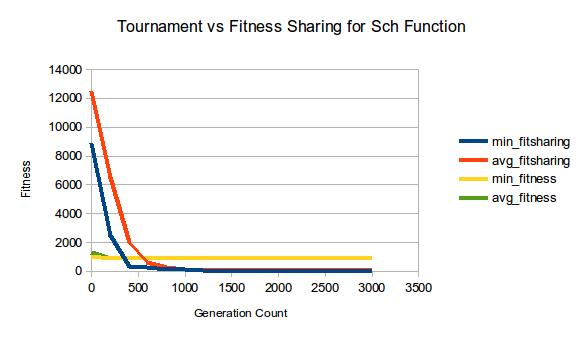
\includegraphics[width=.9\linewidth]{./indi.jpg}
\caption{Compare the Tournament selction method and the Roulette Wheel selection method with fitness sharing through two individual runs, and the results show that the fitness sharing do help find the solution faster indicated by two two individual (no repeats) runs.}
\end{figure}
Compared with the Generational Algorithm, Steady-state Algorithm is very slow because during each generation change, only the worst two population individuals got crossover and mutated with certain rates at each step.

But due to the fact that each generation when I generate the new generation, I almost always (because the crossover rate I have used for this project is 0.9) crossover the sample elite parent and mutated them to replace the population worst two individuals. The worst ones were kicked out of the population pretty fast, so it helps to make average fitness converges fast.

From Figure 1, we can see that at least for these two individual runs (no repeats), the fitness sharing method greatly helped facilitate the evolving process because of the parent selected are better then the ones that could be selected by the Tournament selection method. 
\subsection{Generation vs Population Size}
\label{sec-3-2}

Because of the randomness of the population generation, I mean to repeat each different population size and generation count for 1000 times just like we have done in project 1. But due to the computation complexity of fitness sharing, it took too much time getting the results I want. So instead, I repeated the processes for 100 times and 300 times respectively to compare the results. 

\subsubsection{100 repeats}
\label{sec-3-2-1}

\begin{table}[htb]
\caption{Tournament selection vs Roulette wheel selection with fitness sharing. For each of the 8 combinations, there are 100 repeats to average the results.}
\centering
\begin{tabular}{lrrrr}
\hline
Combination & Minimum & Average & fitShare & fitShare\\
pSize * genCnt & Fitness & Fitness & minFitness & avgFitness\\
\hline
20*1000 & 1158.32886 & 1177.87109 & 487.71091 & 845.61157\\
25*800 & 1048.62195 & 1064.32336 & 296.60168 & 655.26294\\
50*400 & 655.84717 & 663.36511 & 180.82184 & 339.57751\\
100*200 & 400.42111 & 700.03040 & 3535.18530 & 6833.67480\\
200*100 & 2870.95752 & 8169.49365 & 6696.13135 & 11020.54004\\
400*50 & 5994.97217 & 11723.91602 & 7830.01807 & 12106.94238\\
800*25 & 7170.14111 & 12341.81934 & 8331.73145 & 12426.48340\\
1000*20 & 7433.84424 & 12417.54297 & 8601.79004 & 12474.12891\\
\hline
\end{tabular}
\end{table}

\begin{figure}[htb]
\centering
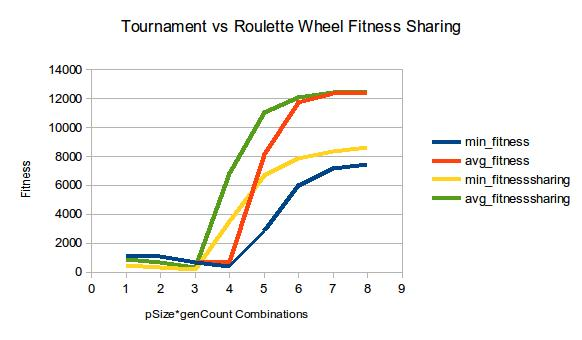
\includegraphics[width=.9\linewidth]{./c100.jpg}
\caption{Tournament selection vs Roulette wheel selection with fitness sharing applied with repeats of 100 to compare the results of searching global optima for the Schwefel Function. (1, 2, 3, \ldots{}, 8 represents 20*1000, 25*800, \ldots{} , 1000*20 as shown in the table respectively. )}
\end{figure}
From the above Table 2 and Figure 2, we can see that the fitness sharing technique slightly improved the minimum fitness and average fitness when the Population size is relatively small, and when Population size increases, and the generation counts reduced, the fitness sharing does not seem to improve the results compared with the general Tournament Selection methods.
And I am wondering if it is because of the limited repeats of only 100. So to see if it makes any difference, I repeated the combinations with the repeats of 300 instead, and the results are listed followed. 
\subsubsection{300 repeats}
\label{sec-3-2-2}

\begin{table}[htb]
\caption{Tournament selection vs Roulette wheel selection with fitness sharing. For each of the 8 combinations, there are 300 repeats to average the results.}
\centering
\begin{tabular}{lrrrr}
\hline
Combination & Minimum & Average & fitShare & fitShare\\
pSize * genCnt & Fitness & Fitness & minFitness & avgFitness\\
\hline
20*1000 & 1203.97180 & 1223.95032 & 564.053 & 898.423\\
25*800 & 1135.35413 & 1151.29761 & 375.123 & 681.101\\
50*400 & 615.35120 & 623.60419 & 227.569 & 436.058\\
100*200 & 358.84329 & 670.93530 & 3724.36 & 6908.23\\
200*100 & 2821.65039 & 8213.76367 & 6753.03 & 11040.00\\
400*50 & 6103.94922 & 11727.93945 & 7774.75342 & 12114.95703\\
800*25 & 7246.77344 & 12345.82129 & 8388.77246 & 12428.90430\\
1000*20 & 7553.78076 & 12420.46582 & 8489.90137 & 12471.96484\\
\hline
\end{tabular}
\end{table}

\begin{figure}[htb]
\centering
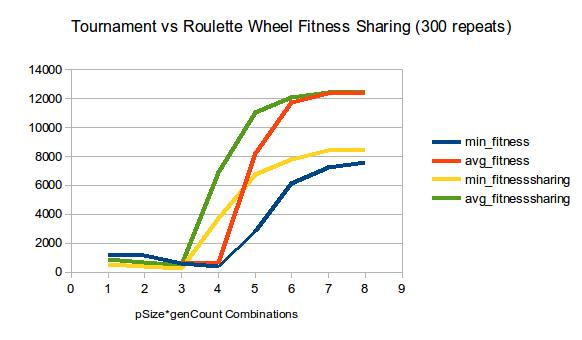
\includegraphics[width=.9\linewidth]{./c300.jpg}
\caption{Tournament selection vs Roulette wheel selection with fitness sharing applied with repeats of 300 to compare the results of searching global optima for the Schwefel Function. (1, 2, 3, \ldots{}, 8 represents 20*1000, 25*800, \ldots{} , 1000*20 as shown in the table respectively. )}
\end{figure}

From the above Table 3 and Figure 3, we can see the results are pretty similar with the 100 repeats. Try to understand the reason why the fitness sharing method helps only for the first 3 combinations, I looked carefully into the three table and figure results. Table 1 and Figure 1 shows that the fitness sharing helps when the Steady-state generation counts reached up to about several hundred to about 1000 generations. But for latter pSize*genCnt combinations, the generation counts are dramatically reduced which means the fitness sharing modules were not able to function yet and the Steady-state algorithm finished already. So for the later 4-5 combinations, the fitness sharing modules showed its influence by mutate tiself from functioning, which also indicates that the fitness sharing does help facilitate the evolving process in finding the global optima for the Schwefel function. 

From the above Table 2 - Table 3 and Figure 2 - Figure 3 results, we can clearly see that there are significant relationship between generations and the population size. As more clearly indicated by the Rastrigin function and the Schwefel function than others, the population size of 100 combined with generation count of 200 uniformly performs the better throughout all these six functions.

This result does not necessarily mean that every time we should choose these kind of numbers, but rather simply indicates the relationship exists. Since any other factors are all kept the same, in reality, when we need to choose reasonable as well as good and efficient numbers, we should conduct similar pretests to tune the factor values a little bit before we start.
\section{Conclusions}
\label{sec-4}
The steady-state genetic algorithm that I have used in this project performs pretty good to solve the Schwefel Function problem that is difficult for regularly-based methods. Compared with project 1a and 1b, by using hill climbing, we could be possibly blocked in local optimum. On the other side, the genetic algorithm can always find the global optimum whenever it takes, it will find it. And actually by applying some scaling factor or tricks, it behave actually pretty good, not taking that long, and it's quite fast and efficient. 

But still, steady-state algorithm should be slightly slower compared with generational algorithm.

There are strong relationship between generation counts and the population size. We don't want population size too small, which could easily result in bias, yet we don't want it to be too large not necessarily slow down the process. Before the initial projects, we should have similar pretests for project design.

By comparing the Tournament selection method and the Roulette Wheel selection methods both by Individual runs without repeats and the repeated runs for 100 and 300 repeats repectively, all the results show that the fitness sharing Function does help in finding the Schwefel Function global optima, just that indicating the help in opposite ways. When the combination has enough generation count for fitness sharing to fully Function, the fitness sharing helps a lot in the result; and when there are not enough generations for fitness sharing to function, the fitness sharing does not help at all, which also indicates its importance and help in this Schwefel Function problem. 
% Emacs 24.3.50.1 (Org mode 8.2.5h)
\end{document}